% !TEX root = ../main.tex
\section{Experimental Results}

The key problem we are trying to resolve is the localization accuracy of Apriltags in noisy situations. Therefore, we want to test the resilience of our algorithm and show that it can obtain reasonable pose estimations under high level of noise. Figure \ref{fig:result_compare} demonstrates a result    We also compare our method against \textit{ar\_track\_alvar}, a popular ARTag detection package that incorporated depth information. Finally, we briefly tested the runtime of the algorithm to show that it remains capable of real time detection. 


\begin{figure}[h]
\centering
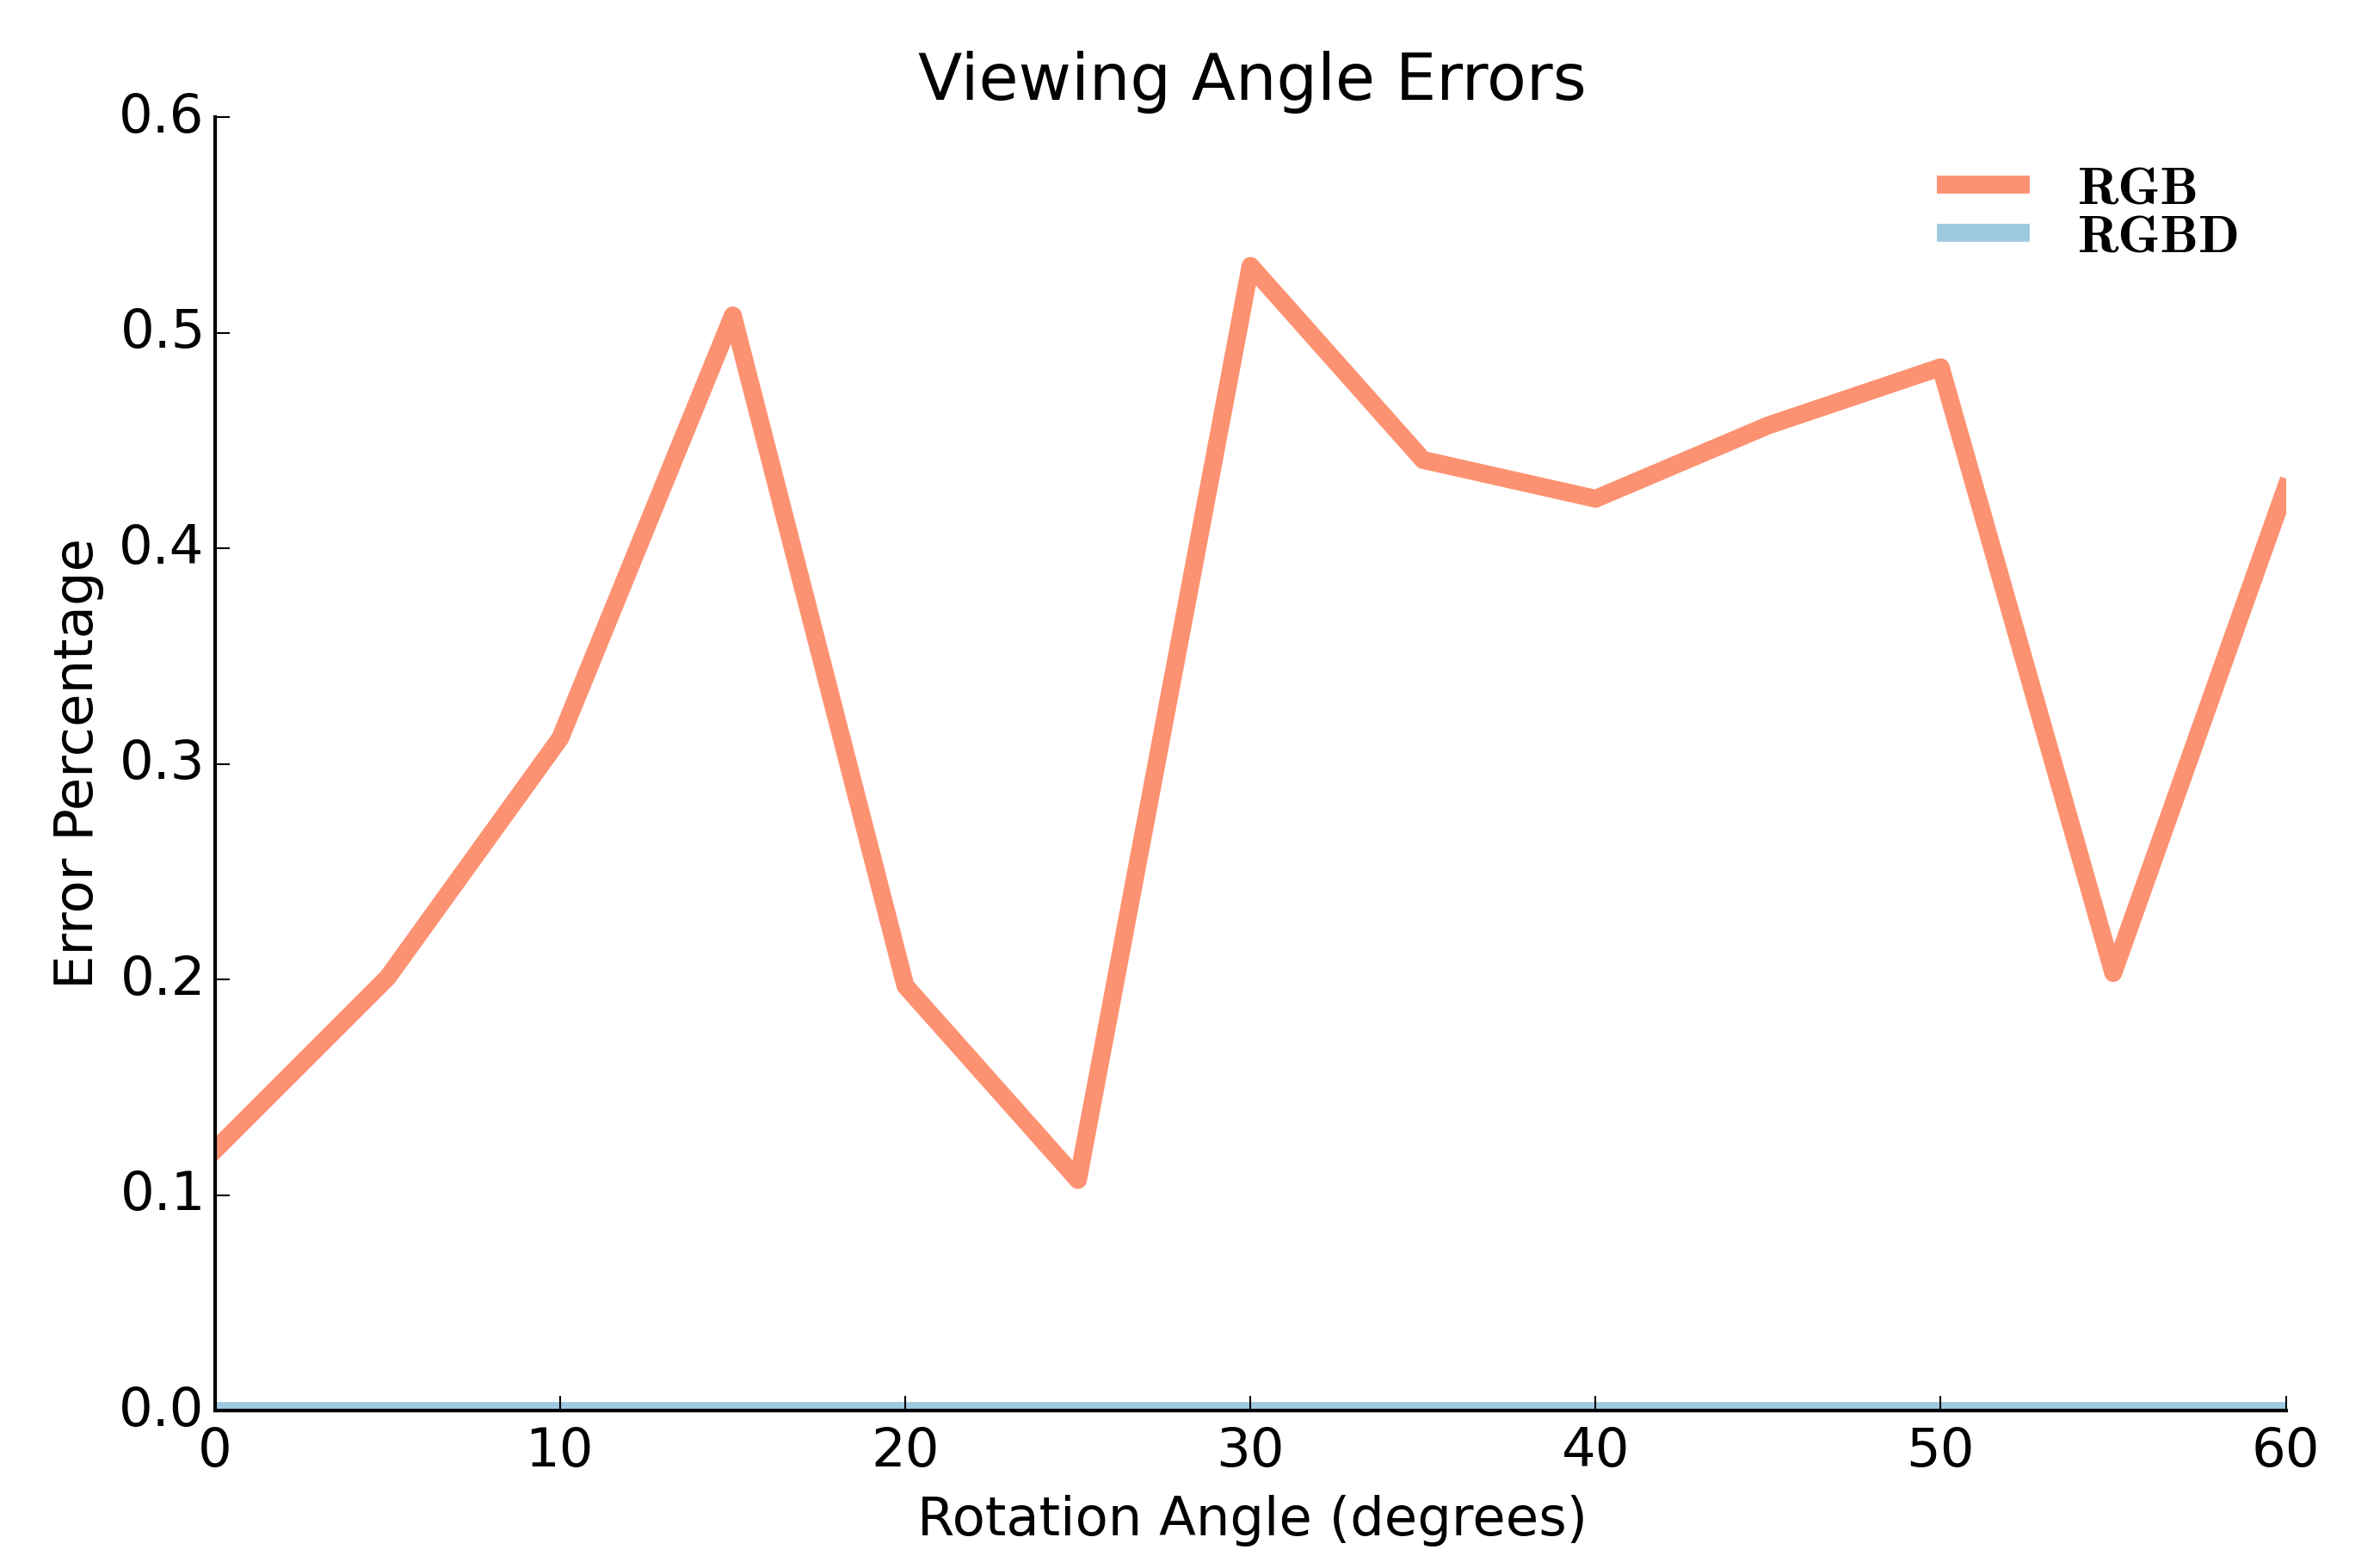
\includegraphics[width=\columnwidth, height=130px]{figs/viewing_angle_fig2}
\caption{Viewing Angle vs Error Percentage under different simulated noise level. The new RGBD based algorithm can resist noise in the RGB image and it vastly outperforms the original algorithm.}
\label{fig:viewing_result}
\end{figure}

In our experiments, we measured the rotational and translation accuracy of the detection algorithms with respect to three different independent variables: viewing angles, distances, and lighting conditions. We placed a standard camera calibration chessboard and an Apriltag of known size on a solid planar board. The Apriltag has a fixed distance from the chessboard. This is used to compute the ground-truth pose for the tag. By using a large chessboard, we can detect the corners to a sub-pixel accuracy and compute accurate ground-truth poses unsusceptible to lighting and sensory noises. 

\subsection{Viewing Angle}

\begin{figure}
\centering
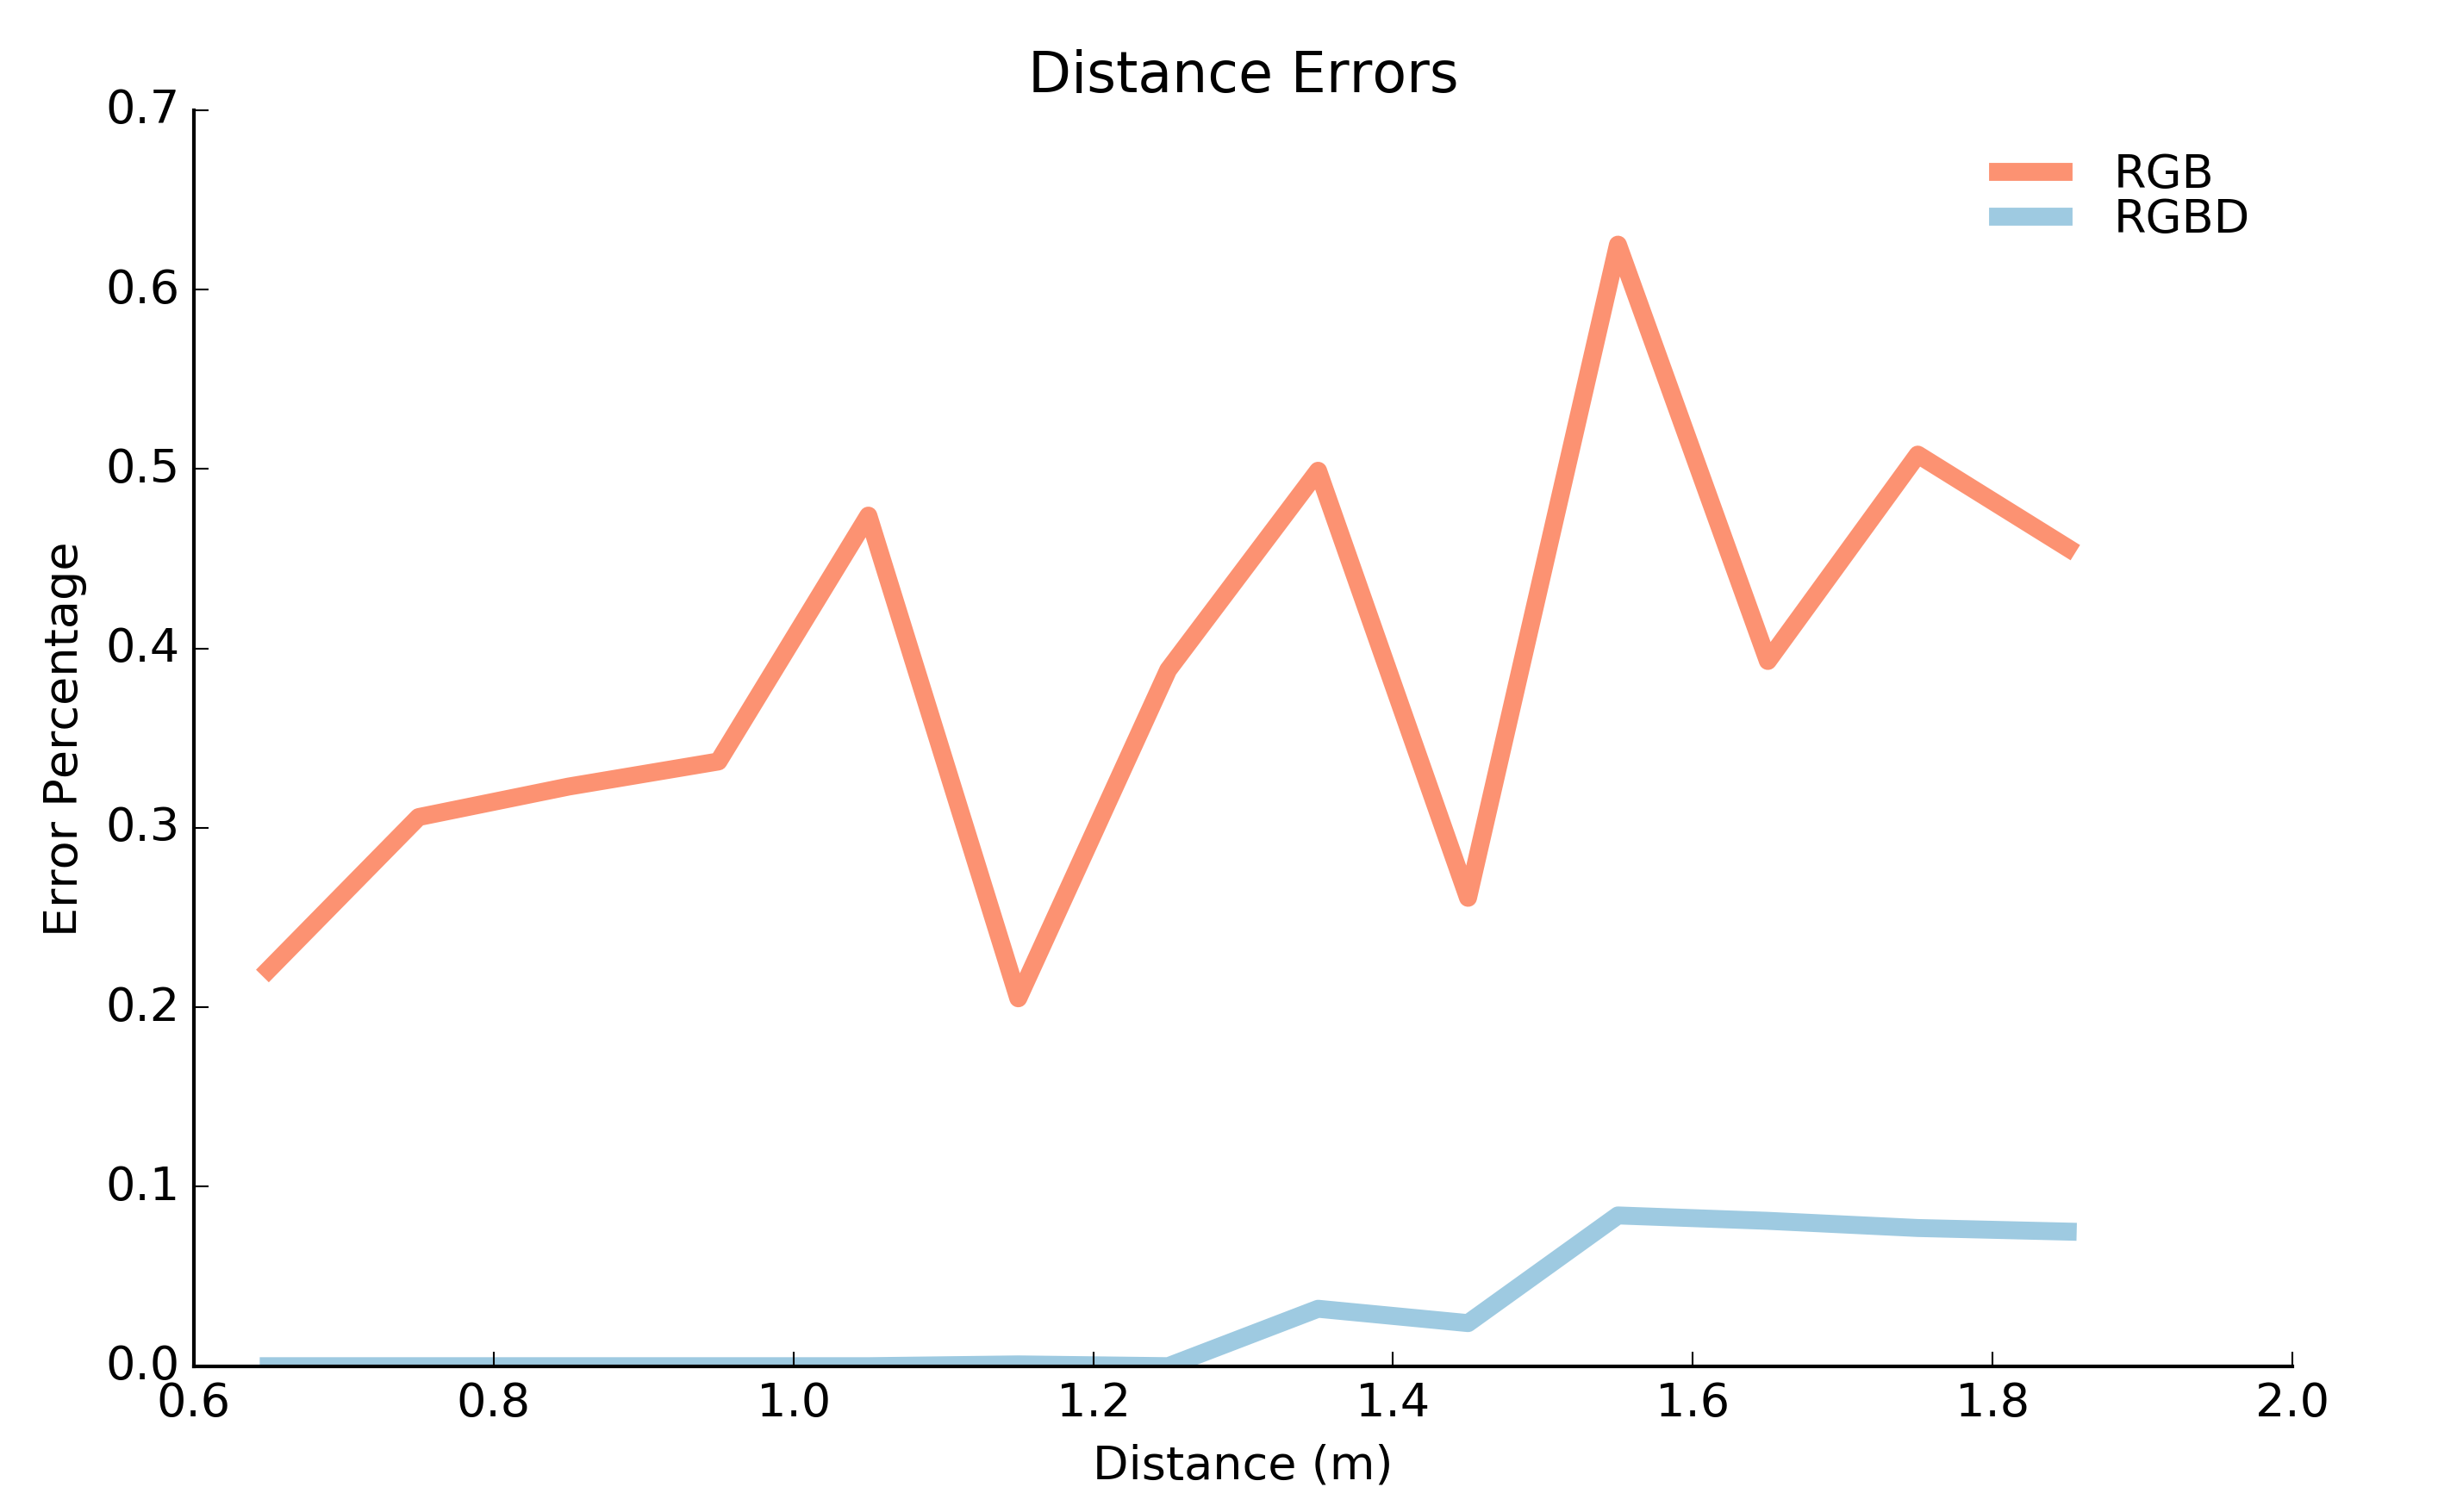
\includegraphics[width=\columnwidth]{figs/distance_fig2}
\caption{Distance vs Error Percentage. Data are captured at a $10$ cm increment from $65$ cm to $185$ cm.}
\label{fig:distance_result}
\end{figure}

Due to the perspective ambiguity effect, the localization accuracy of the Apriltags is heavily affected by the viewing angle of the tag. To characterize the effect, we placed the testing board on a table straight in front of the robot as shown in \ref{fig:exp_setup}. Since the sensor is taller than the plane of the table, the robot has to slightly gaze down at it. We placed the testing board ~$0.65$ meters away from the sensor and rotated it at a increment of 5 degrees from 0 degrees to 60. The angles are measured from the axis parallel to the sensor. This is about the range which the tag can be detected reliably given the camera resolution and the distance. At each angle, we captured the RGB image, depth image, and detection outputs from the Apriltag library. 

For each captured data bundle, we introduced 3 levels of Gaussian noise of $\sigma = 0.2$, $\sigma = 0.5$, $\sigma = 1$  to the RGB image and computed the resulting tag pose. This is repeated for $1000$ trails for each data bundle per noise level and the errors are computed for each trial.  

The empirical result in Figure \ref{fig:bimodal} show a very clear bimodal distribution, as we expected, for the detected poses for a given data bundle over $1000$ trials. In Figure \ref{fig:viewing_result}, we threshold all the poses based on their rotational errors and plotted the percentage of unacceptable poses at each viewing angle. The proposed RGBD fused algorithm vastly outperforms the original algorithm as it has better localization accuracy at all viewing angles and noise levels. 

\subsection{Distance}

%To test the estimation accuracy with respect to distance, we captured the images at different distances away from the camera at a fixed angle. Figure \ref{fig:distance_result} shows the experiment results.
The relationship between the distance and localization accuracy is much more apparent. As the tag moves further away from the sensor, the number of pixels on the tag decreases. The perspective ambiguity effect becomes more apparent when there is only a small patch of pixels on the tag. We show the results of  both RGB and RGBD methods in Figure \ref{fig:distance_result}. During the experiment, it is difficult to keep the viewing angle precisely consistent at each trail. Therefore, the pose error percentage using RGB is not increasing smoothly as they are in the simulation results.

We see a clear increase in error percentage in the proposed method when the tag is far away from the camera. This is contributed both by a smaller tag patch size in the depth image and an increase in noise with the Kinect sensor at a further distance. In these cases, the variance of the depth plane estimation becomes very wide and the algorithm is unable to converge to the correct pose. Nevertheless, our method shows a significant gain in accuracy at every distance.

\subsection{Lighting}

\begin{figure}
\centering
\subfloat[Dark]{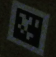
\includegraphics[width=50px, height=50px]{figs/illumination/dark}}
\subfloat[Dim]{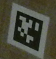
\includegraphics[width=50px, height=50px]{figs/illumination/dim}}
\subfloat[Normal]{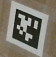
\includegraphics[width=50px, height=50px]{figs/illumination/normal}}
\subfloat[Bright]{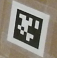
\includegraphics[width=50px, height=50px]{figs/illumination/bright}}
\caption{Apriltags captured by Kinect V2 under different levels of illumination. The RGB sensor dynamically adjust the exposure time to compensate for low lighting. In (a), the image is captured outside of Kinect's adjustable range and the pixels are underexposed. In (b), the long exposure time introduced noticeable noise to the image. }
\label{fig:illumination_tag}
\end{figure}

\begin{figure}[h]
\centering
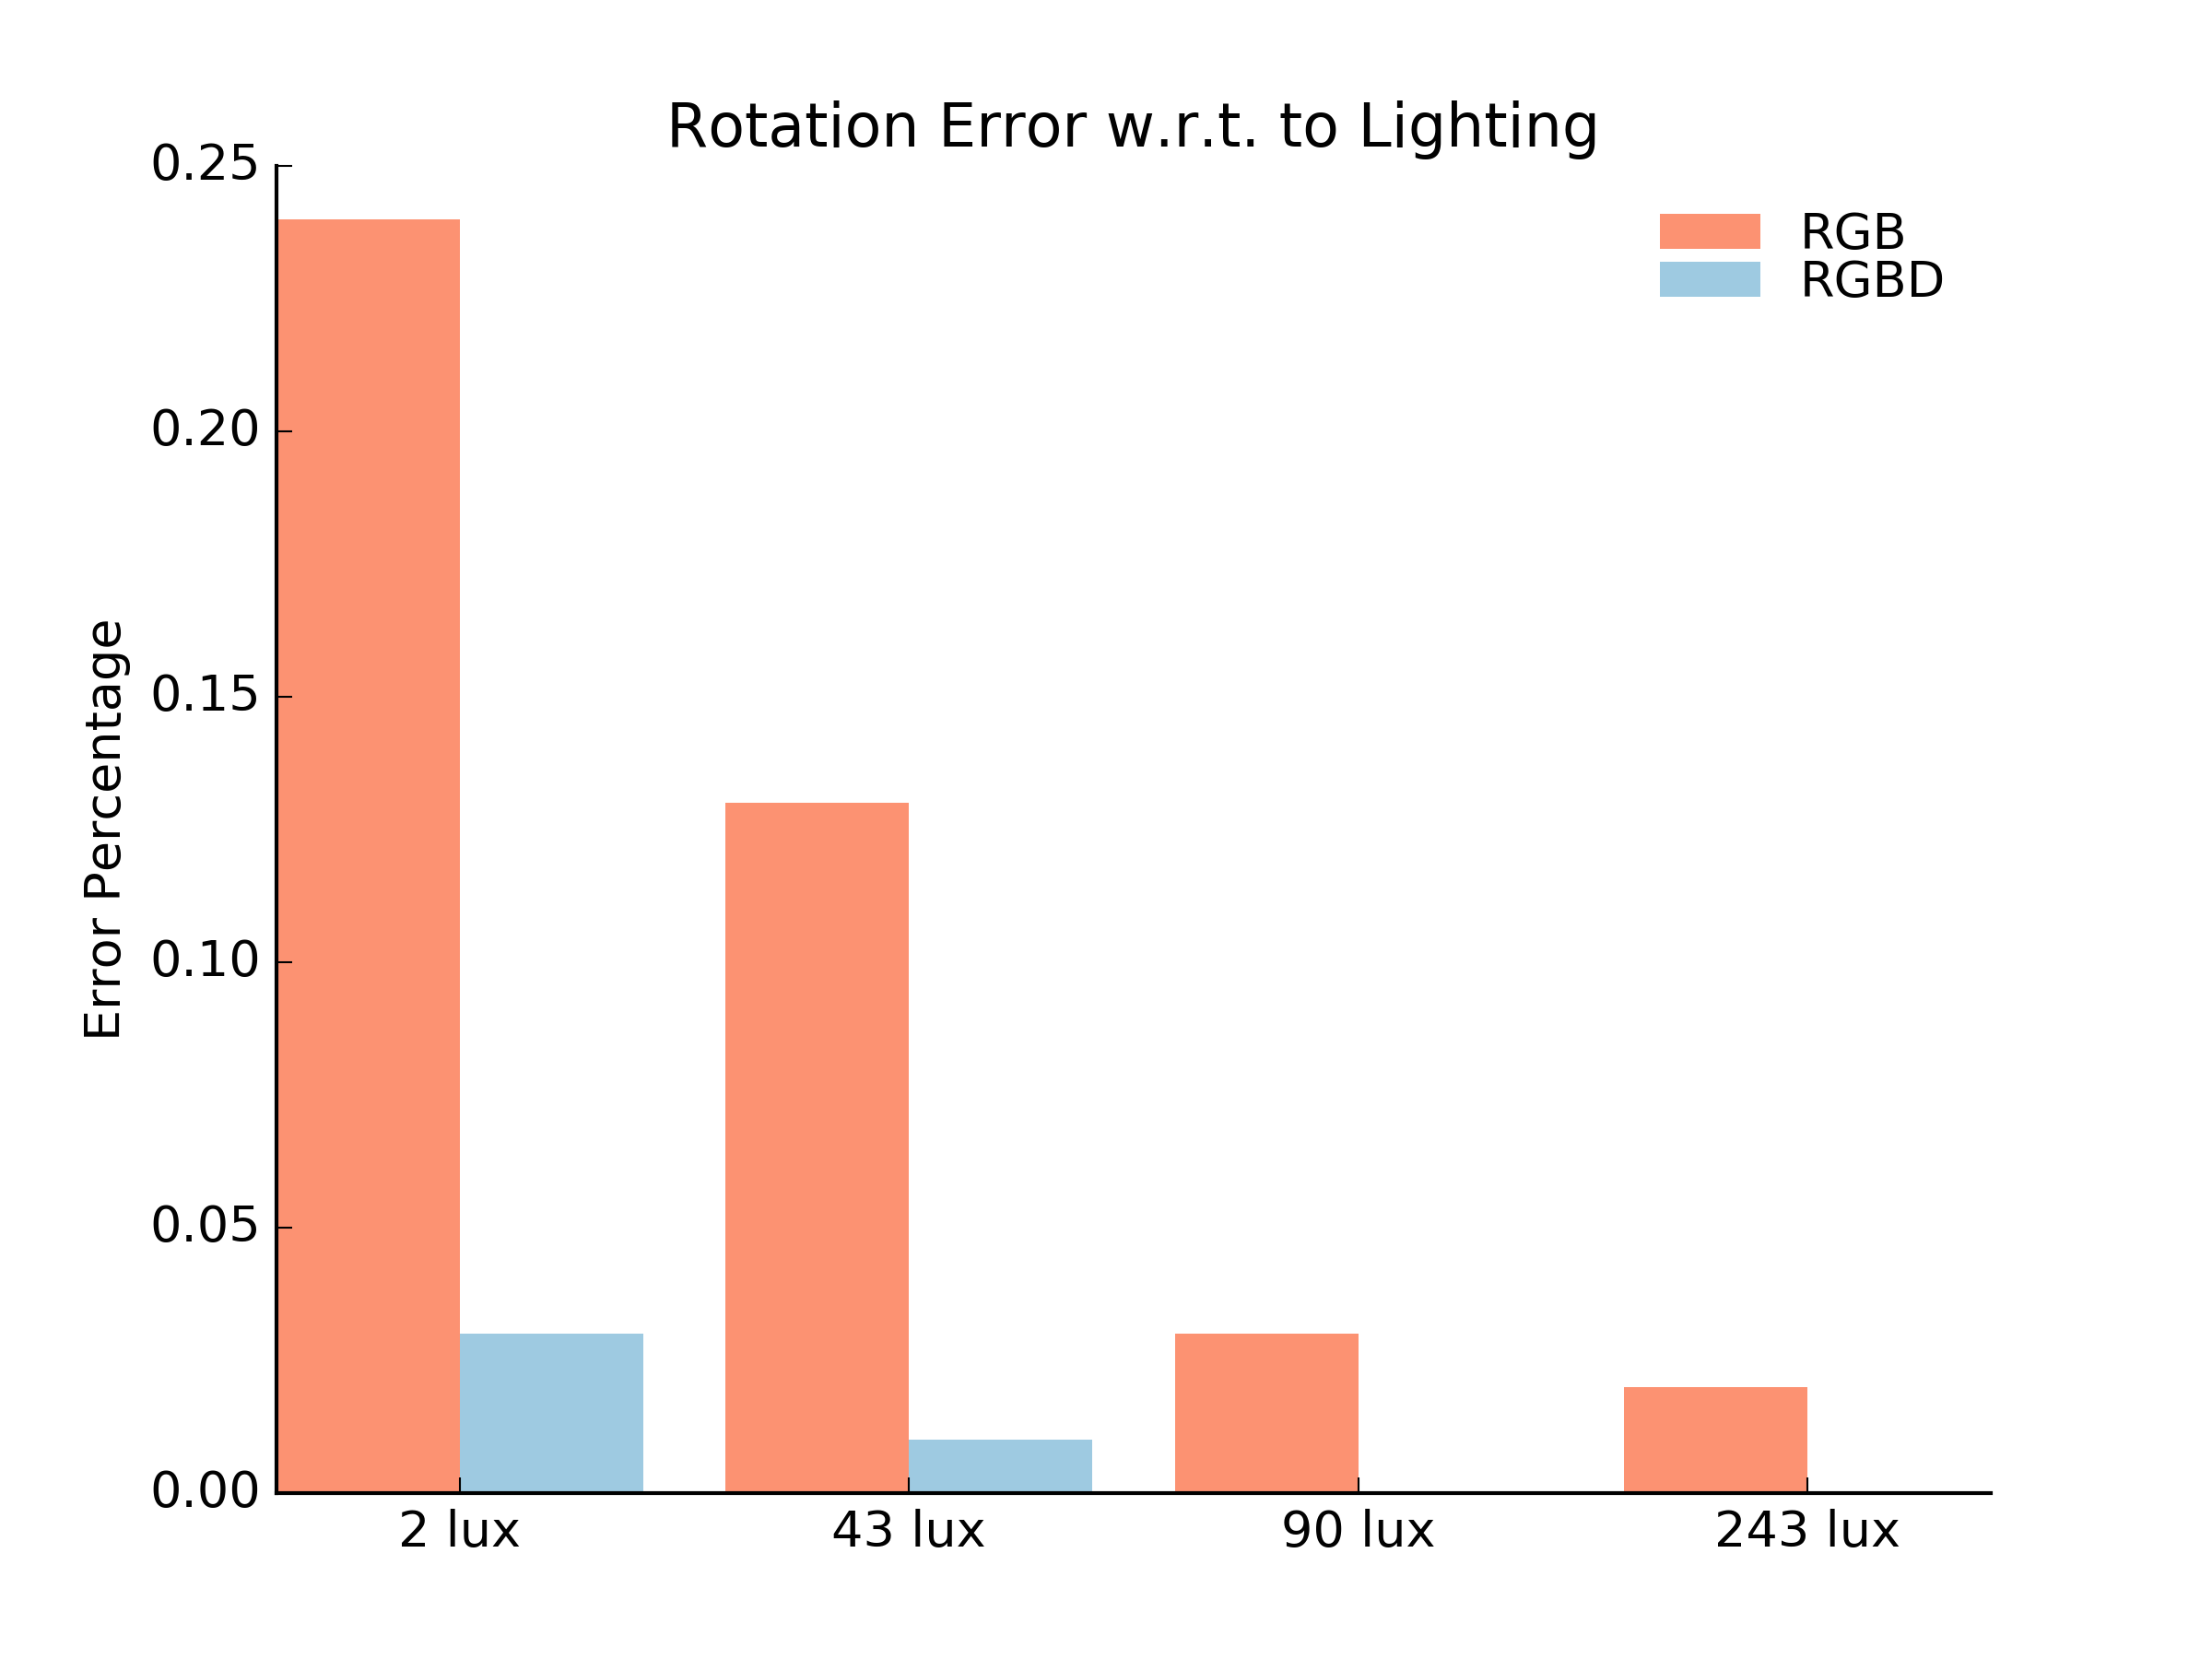
\includegraphics[width=\columnwidth]{figs/lighting_fig1}
\caption{Illumination vs Error Percentage. Data are captured at $65$ cm away from the camera at a $40$ degree angle.}
\label{fig:lighting_result}
\end{figure}

From our past observations, poor lighting condition is the most significant contributing factor to noise and it results in low localization accuracy. The Kinect V2 sensor used in our experiments dynamically adjust the exposure time under low lighting conditions. When pictures are taken below or near the adjustable range of the sensor, they contain very noticeable noise as shown in Figure \ref{fig:illumination_tag}.

We also tested the algorithm under harsh lighting conditions in a real world setting. The data were captured under 4 different lighting conditions: 20 lux (dark), 43 (lux) dim, and (90 lux) normal, 243 lux (bright). We recorded a static scene over 5 seconds and randomly sampled 100 frames to run the test.  As results shown in Figure \ref{fig:lighting_result}, the localization accuracy significantly improves with better illumination. At the lowest illumination, nearly $25\%$ of the poses were unacceptable (more than $20$ degrees off) at the particular viewing angle. By using depth sensor which is unaffected by poor source radiance, there are only ~$3\%$ of unacceptable poses.

\subsection{Benchmark Against ar\_track\_alvar}

\begin{figure}
\centering
\subfloat[Rotation Error]{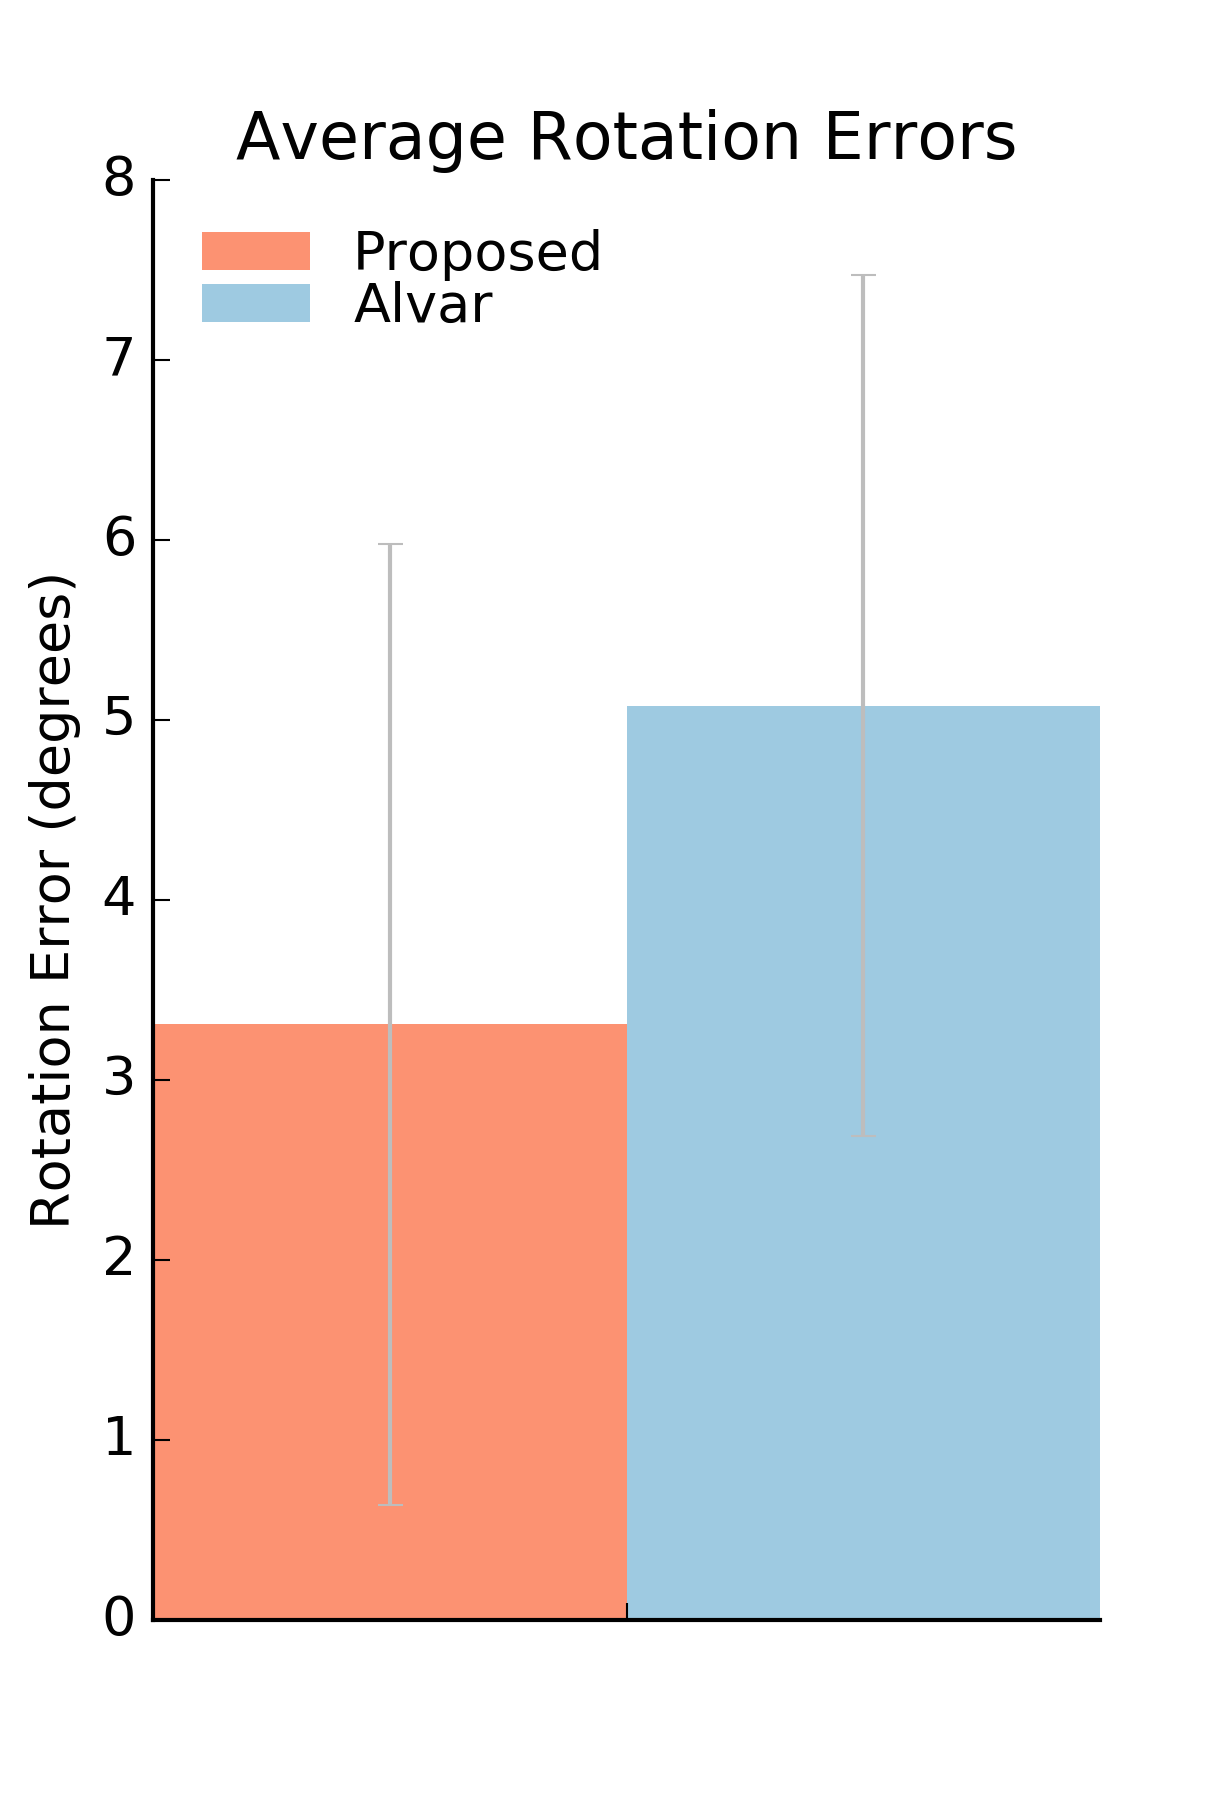
\includegraphics[width=120px, height=180px]{figs/alvar_rot}}
\subfloat[Translation Error]{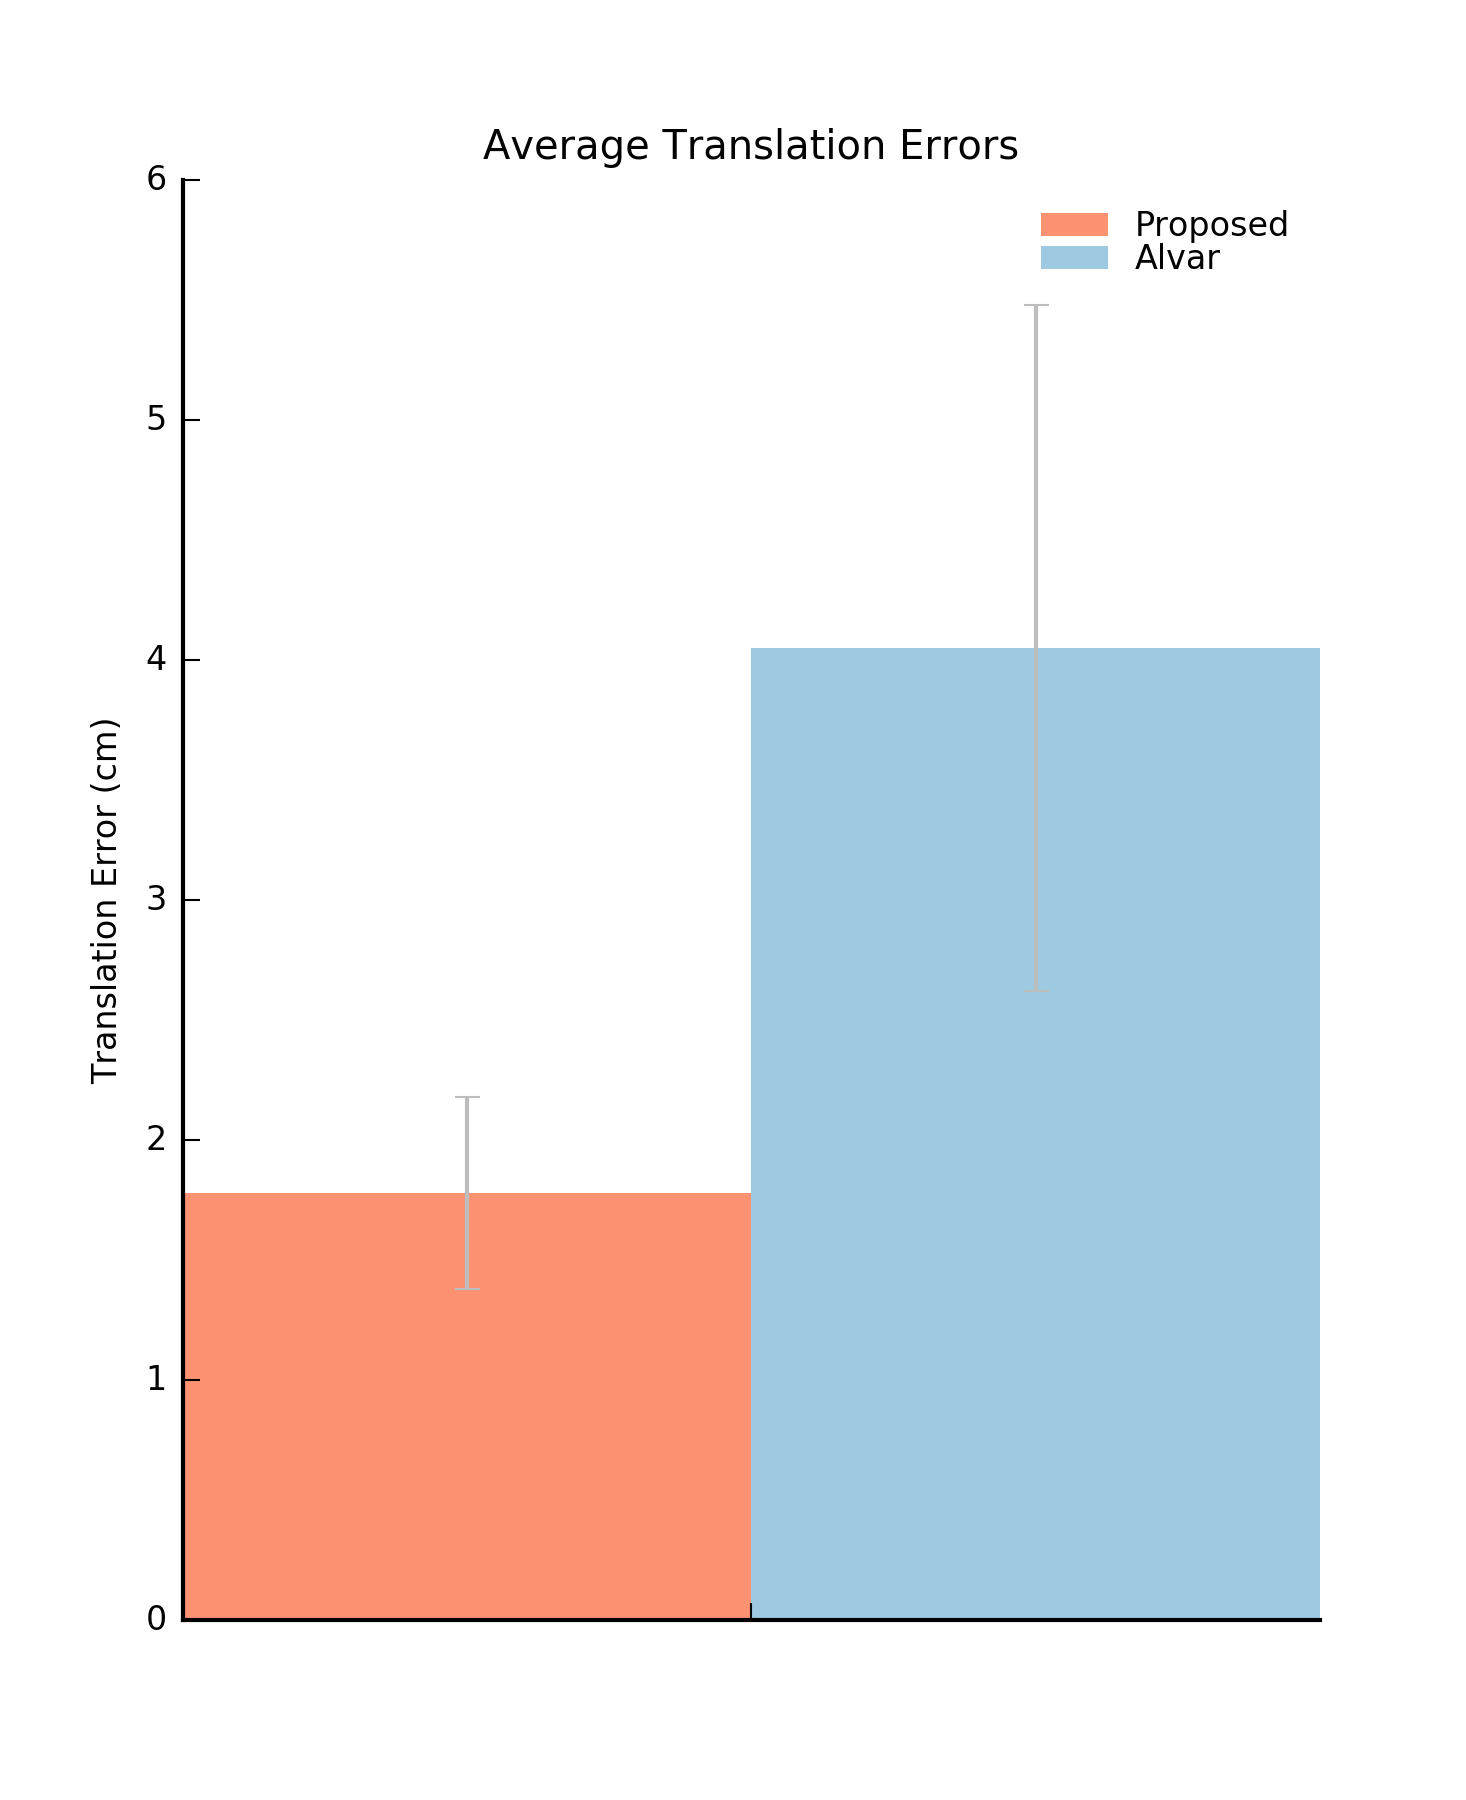
\includegraphics[width=120px, height=180px]{figs/alvar_trans}}
\caption{Average pose errors compared with ar\_track\_alvar package.}
\label{fig:alvartrack}
\end{figure}

ar\_track\_alvar is a ROS wrapper package for Alvar [], an open source AR tag tracking library. The package is designed for AR tag detection and pose estimation for robots similar to Apriltags. In particular, it implements a module where depth sensor is integrated to improve the pose estimation. The package use the detected corner points to extract a patch of point clouds containing the tag. Then it proceed to fit a plane of the point cloud data and find its centroid using PCL. The pose of the tag is computed by aligning the centroid with the center of the tag.   

We implemented a similar module for the Apriltag and compared the pose accuracy between our proposed method and the module using all the collected data. The results are shown in Figure \ref{fig:alvartrack}. The two algorithms performed similarly in rotation error, but the proposed method was on average $2$ cm better with the position component. The spread of error is also much smaller for the position component indicating that our purposed method is more consistent.

\subsection{Computation Time}
We briefly tested the computation time of the new algorithm. With our current implementation in Python, the additional computation time for sensor fusing process is ~$11$ ms. Therefore the entire detection pipeline can process a $960$ x $540$ image within $35$ ms. All tag detectors and the fusing process were running in a single-threaded mode of an Intel core. Since our sensory updates at roughly $35Hz$, the entire pipeline can process the tags and estimate the pose in near real time. There is no significant time increase on a higher resolution image for the fusing process because our algorithm does not need to process the entire image.

The most time consuming step is running the trust region optimization for refining the pose. This process can be sped up significantly by simply implementing the pipeline in C++.